%----------------------------------------------------------------------

\documentclass[
	layoutmode=block,
	% make the spread 16x9...
	blockwidth=96mm, blockheight=108mm,
	bleed=0mm,
	bindingoffset=0mm,
	% image block configuration...
	imageblockwidth=0.98, imageblockheight=0.98,
	imageblockoffsettop=0mm,
	% misc...
	12pt,final,openany
]{photobook}

%\usepackage{xcolor}
%\usepackage{pagecolor}
\usepackage{anyfontsize}
\usepackage{ragged2e}
\usepackage{hyperref}
\usepackage{cprotect}

%\usepackage{listings}
\usepackage{fancyvrb}

\usepackage{ccicons}
\usepackage{lipsum}



% - - - - - - - - - - - - - - - - - - - - - - - - - - - - - - - - - - -

\setlength\parindent{0pt}

\writeimagelistfalse

\pagestyle{empty}

\pagecolor{white}


%\fontsize{30pt}{36pt}\selectfont

% fonts...
\usepackage{fontspec}
\setmainfont[Mapping=tex-text]{Open Sans}
\setsansfont[Mapping=tex-text]{Open Sans}
%\setmonofont[Mapping=tex-text, Scale=0.8]{Courier New}
\newfontfamily\titlefont[Mapping=tex-text]{Open Sans Light}
\newfontfamily\sectiontitlefont[Mapping=tex-text]{Open Sans Light}

\def\captionsize{%
	\fontsize{4pt}{5pt}\selectfont}


% - - - - - - - - - - - - - - - - - - - - - - - - - - - - - - - - - - -
% Macros/templates...

\def\TEX{%
	{\fontfamily{lmr}\selectfont \TeX}}
\def\LATEX{%
	{\fontfamily{lmr}\selectfont \LaTeX}}

\newcommand\PageFushRight[1]{
	\begin{page}
		\begin{cell}{2mm,2mm}{\paperwidth - 4mm}{\paperheight - 4mm}
			\begin{flushright}
				#1
			\end{flushright}
		\end{cell}
	\end{page}}
\newcommand\PageFushLeft[1]{
	\begin{page}
		\begin{cell}{2mm,2mm}{\paperwidth - 4mm}{\paperheight - 4mm}
			\begin{flushleft}
				#1
			\end{flushleft}
		\end{cell}
	\end{page}}

\newcommand\PageFushRightC[1]{
	\begin{page}
		\begin{cell}{2mm,2mm}{\paperwidth - 4mm}{\paperheight - 4mm}
			\null
			\vfill
			\begin{flushright}
				#1
			\end{flushright}
			\vfill
			\null
		\end{cell}
	\end{page}}
\newcommand\PageFushLeftC[1]{
	\begin{page}
		\begin{cell}{2mm,2mm}{\paperwidth - 4mm}{\paperheight - 4mm}
			\null
			\vfill
			\begin{flushleft}
				#1
			\end{flushleft}
			\vfill
			\null
		\end{cell}
	\end{page}}




\begin{document} %-----------------------------------------------------

% cover...

\ImagePageClear[clearance=28mm]{%
	\begin{minipage}{\cellwidth}
		\vspace{-1mm}
		\begin{center}
			\color{lightgray}
			\hspace{-1.7mm}This is not a presentation, it's a well camoflaged book
		\end{center}
	\end{minipage}}{images/DSC00182}


% - - - - - - - - - - - - - - - - - - - - - - - - - - - - - - - - - - -
% title...

\ImageSpread[clearance=40mm]{}{images/latex}


% - - - - - - - - - - - - - - - - - - - - - - - - - - - - - - - - - - -
% history...

\PageFushRight{
	\null
	\vfill
	\vspace{-12mm}
	\section*{1978: TeX}%
	\vspace{-4mm}
	Donald Knuth

	\section*{1984: LaTeX}%
	\vspace{-4mm}
	Leslie Lamport
	\vfill
	\fontsize{4pt}{5pt}\selectfont
	\textbf{2021: photobook}

	\fontsize{3.5pt}{4.5pt}\selectfont
	Alex A. Naanou}

\PageFushLeft{
	\null
	\vfill
	\vspace{12mm}
	\section*{1982: PostScript}%
	\vspace{-4mm}
	%John Warnock, Chuck Geschke, Doug Brotz, Ed Taft, Bill Paxton
	Adobe Systems

	\section*{1993: PDF}%
	\vspace{-4mm}
	Adobe Inc.
	\vfill
	\null}


% - - - - - - - - - - - - - - - - - - - - - - - - - - - - - - - - - - -
% hello world...

\begin{page}%
\scriptsize%
\vfill%
\begin{center}%
\BVerbatimInput{hello-world.tex}
\end{center}%
\vfill%
\end{page}
%
\pagecolor{lightgray}
\ImagePageClear{}{hello-world}
\pagecolor{white}


% - - - - - - - - - - - - - - - - - - - - - - - - - - - - - - - - - - -
% text layout...

\begin{spreadtopages}
	\vfill
	\begin{center}
		\section*{Text $+$ Boxes $\longrightarrow$ Pages}
	\end{center}
	\vfill
\end{spreadtopages}
\newpage


% - - - - - - - - - - - - - - - - - - - - - - - - - - - - - - - - - - -
% layout example...

% left page...
\begin{page}
\fontsize{5pt}{5.5pt}\selectfont
\vfill
\begin{center}
\begin{BVerbatim}
Lorem ipsum dolor sit amet, consectetuer adipiscing elit. Ut purus
elit, vestibulum ut, placerat ac, adipiscing vitae, felis. Curabitur
dictum gravida mauris. Nam arcu libero, nonummy eget, consectetuer
id, vulputate a, magna. Donec vehicula augue eu neque. Pellentesque
habitant morbi tristique senectus et netus et malesuada fames ac
turpis egestas. Mauris ut leo. Cras viverra metus rhoncus sem. Nulla et
lectus vestibulum urna fringilla ultrices. Phasellus eu tellus sit amet
tortor gravida placerat. Integer sapien est, iaculis in, pretium quis,
viverra ac, nunc. Praesent eget sem vel leo ultrices bibendum. Aenean
faucibus. Morbi dolor nulla, malesuada eu, pulvinar at, mollis ac,
nulla. Curabitur auctor semper nulla. Donec varius orci eget risus.
Duis nibh mi, congue eu, accumsan eleifend, sagittis quis, diam. Duis
eget orci sit amet orci dignissim rutrum.

Nam dui ligula, fringilla a, euismod sodales, sollicitudin vel,
wisi. Morbi auctor lorem non justo. Nam lacus libero, pretium at, lobortis
vitae, ultricies et, tellus. Donec aliquet, tortor sed accumsan bibendum,
erat ligula aliquet magna, vitae ornare odio metus a mi. Morbi ac orci et
nisl hendrerit mollis. Suspendisse ut massa. Cras nec ante. Pellentesque
a nulla. Cum sociis natoque penatibus et magnis dis parturient montes,
nascetur ridiculus mus. Aliquam tincidunt urna. Nulla ullamcorper
vestibulum turpis. Pellentesque cursus luctus mauris.
\newpage
\end{BVerbatim}
\end{center}
\vfill
\null
\end{page}

% right page...
{\tiny%
	Lorem ipsum dolor sit amet, consectetuer adipiscing elit. Ut purus
	elit, vestibulum ut, placerat ac, adipiscing vitae, felis. Curabitur
	dictum gravida mauris. Nam arcu libero, nonummy eget, consectetuer
	id, vulputate a, magna. Donec vehicula augue eu neque. Pellentesque
	habitant morbi tristique senectus et netus et malesuada fames ac
	turpis egestas. Mauris ut leo. Cras viverra metus rhoncus sem. Nulla et
	lectus vestibulum urna fringilla ultrices. Phasellus eu tellus sit amet
	tortor gravida placerat. Integer sapien est, iaculis in, pretium quis,
	viverra ac, nunc. Praesent eget sem vel leo ultrices bibendum. Aenean
	faucibus. Morbi dolor nulla, malesuada eu, pulvinar at, mollis ac,
	nulla. Curabitur auctor semper nulla. Donec varius orci eget risus.
	Duis nibh mi, congue eu, accumsan eleifend, sagittis quis, diam. Duis
	eget orci sit amet orci dignissim rutrum.

	Nam dui ligula, fringilla a, euismod sodales, sollicitudin vel,
	wisi. Morbi auctor lorem non justo. Nam lacus libero, pretium at, lobortis
	vitae, ultricies et, tellus. Donec aliquet, tortor sed accumsan bibendum,
	erat ligula aliquet magna, vitae ornare odio metus a mi. Morbi ac orci et
	nisl hendrerit mollis. Suspendisse ut massa. Cras nec ante. Pellentesque
	a nulla. Cum sociis natoque penatibus et magnis dis parturient montes,
	nascetur ridiculus mus. Aliquam tincidunt urna. Nulla ullamcorper
	vestibulum turpis. Pellentesque cursus luctus mauris.
	\newpage}


% - - - - - - - - - - - - - - - - - - - - - - - - - - - - - - - - - - -
% build...

\begin{spreadtopages}
	\vfill
	\begin{center}
		\section*{.tex $\longrightarrow$ .pdf}
		\vspace{1.5em}
		\hspace{1mm}
		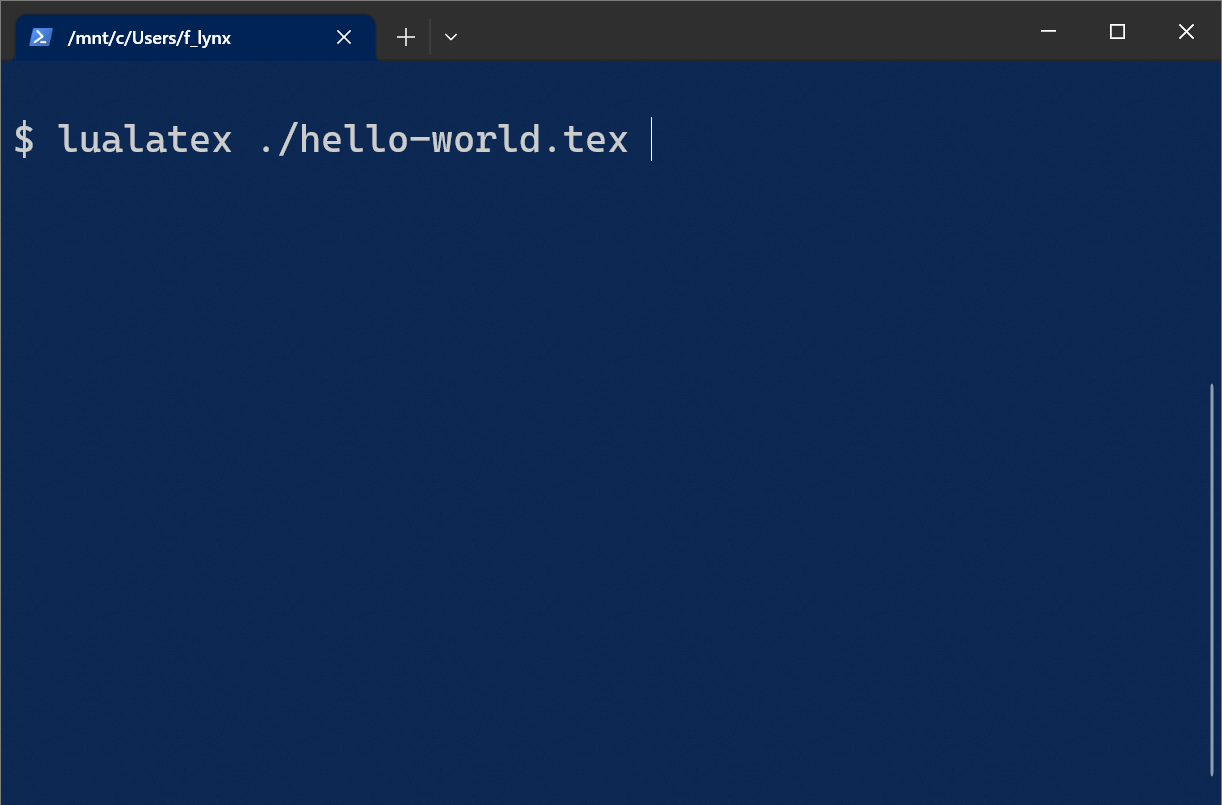
\includegraphics[keepaspectratio, height=0.5\cellheight]{images/commandline}
		\hspace{4mm}
		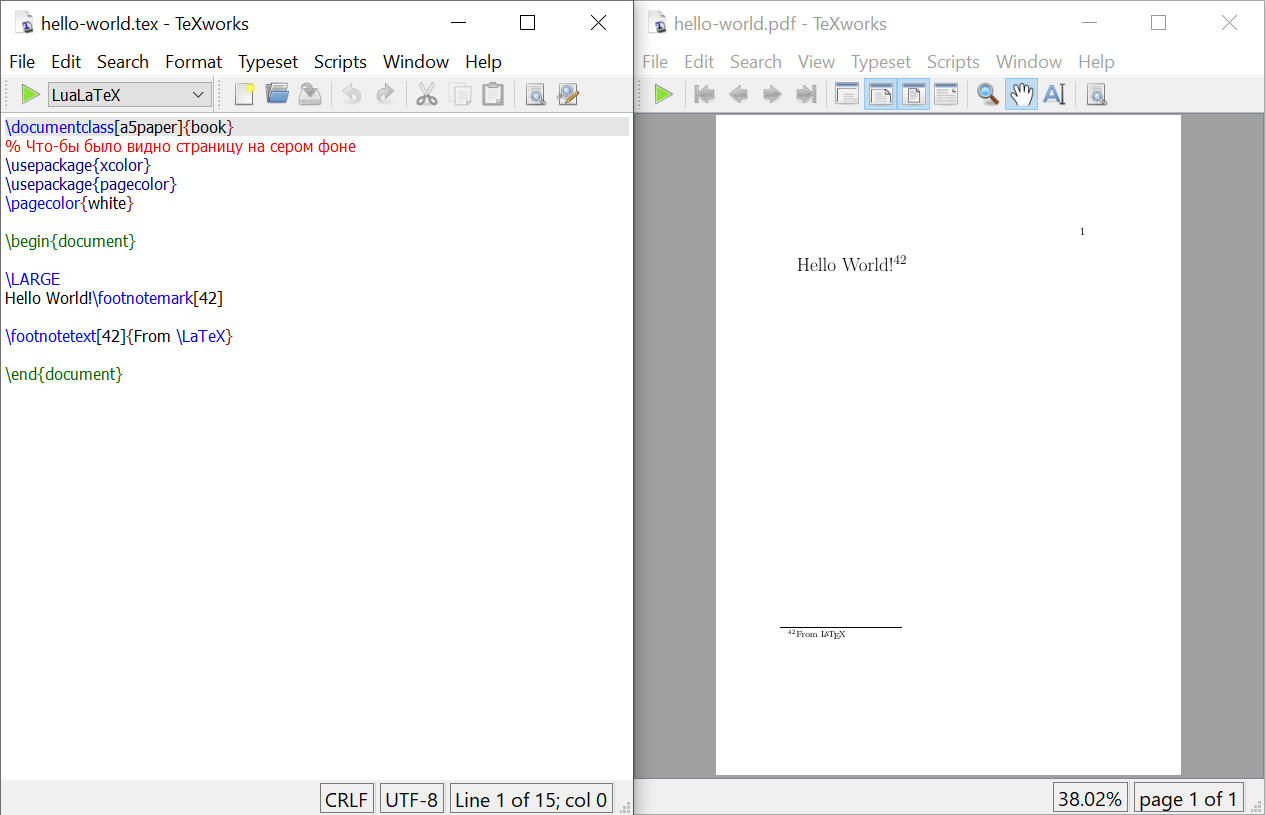
\includegraphics[keepaspectratio, height=0.5\cellheight]{images/TeXWorks}
	\end{center}
	\vfill
\end{spreadtopages}


% - - - - - - - - - - - - - - - - - - - - - - - - - - - - - - - - - - -
% Advantages / disadvanages

\newcommand\seppoints{%
	\par
	\vspace{0.1em}}
\PageFushRightC{
	\section*{Advantages}
	Simple templating
	\seppoints
	Handling large projects
	\seppoints
	Full support for everything needed
	\seppoints
	Documentation
	\seppoints
	Free and open source
}
\PageFushLeftC{
	\vspace{-0.5em}
	\section*{Disadvantages}
	Not WYSIWYG
	\seppoints
	Harder to create graphics
	\seppoints
	Not as efficient for smaller tasks
}


% - - - - - - - - - - - - - - - - - - - - - - - - - - - - - - - - - - -
% Alternatives...

\PageFushRightC{
	\section*{Alternatives}
	\vspace{1em}
	\subsection*{Adobe:}
	\vspace{-.7em}
	InDesign / Illustrator / Photoshop / DPS }
\PageFushLeftC{
	\vspace{-0.5em}
	\subsection*{OpenSource:}
	\vspace{-.7em}
	Scribus / Inkscape / Krita / Blender }


% - - - - - - - - - - - - - - - - - - - - - - - - - - - - - - - - - - -
% photobook...

\begin{spreadtopages}
	\vfill
	\begin{center}
		\fontsize{42pt}{45pt}\selectfont
		photobook
	\end{center}
	\vfill
\end{spreadtopages}


% - - - - - - - - - - - - - - - - - - - - - - - - - - - - - - - - - - -
% differences to native LaTeX...

\PageFushRightC{
	\section*{in photobook}
	\vspace{-7mm}
	we can do:}

\PageFushLeftC{
		Bleeds

		Pages

		Spreads

		Foldouts

		Endpapers

		Covers

		Jackets
}


% - - - - - - - - - - - - - - - - - - - - - - - - - - - - - - - - - - -

\begin{page}
\vfill
\begin{center}
\begin{BVerbatim}
\documentclass{photobook}
\end{BVerbatim}
\end{center}
\vfill
\null
\end{page}

\begin{page}%
\begin{Verbatim}[tabsize=4]
\documentclass[
	layoutmode=block,
	blockwidth=96mm, 
	blockheight=108mm,
	bleed=0mm,
	bindingoffset=0mm,
	imageblockwidth=0.98, 
	imageblockheight=0.98,
]{photobook}
\end{Verbatim}
\end{page}


% - - - - - - - - - - - - - - - - - - - - - - - - - - - - - - - - - - -

\begin{page}%
\vfill%
\begin{center}%
\scriptsize%
\begin{BVerbatim}
\ImagePageClear{Park}{images/DSC03759}
\end{BVerbatim}
\end{center}%
\vfill%
\null%
\end{page}

\ImagePageClear{Park}{images/DSC03759}


% - - - - - - - - - - - - - - - - - - - - - - - - - - - - - - - - - - -

\begin{page}%
\vfill%
\begin{center}%
\scriptsize%
\begin{BVerbatim}
\ImagePageFit{}{images/DSC02091}
\end{BVerbatim}
\end{center}%
\vfill%
\null%
\end{page}

\ImagePageFit{}{images/DSC02091}


% - - - - - - - - - - - - - - - - - - - - - - - - - - - - - - - - - - -

\cprotEnv\begin{spreadtopages}%
\normalsize
\vfill%
\begin{center}%
\begin{BVerbatim}
\ImageSpread{"Копейка под домом"}{images/DSC05647}
\end{BVerbatim}
\end{center}%
\vfill%
\null%
\end{spreadtopages}

\ImageSpread{"Копейка под домом"}{images/DSC05647}


% - - - - - - - - - - - - - - - - - - - - - - - - - - - - - - - - - - -

\cprotEnv\begin{spreadtopages}%
\normalsize
\vfill%
\begin{center}%
\begin{BVerbatim}
\ImageSpreadFitL{New year}{images/DSC03603a}
\end{BVerbatim}
\end{center}%
\vfill%
\null%
\end{spreadtopages}

\ImageSpreadFitL{New year}{images/DSC03603a}


% - - - - - - - - - - - - - - - - - - - - - - - - - - - - - - - - - - -

\cprotEnv\begin{spreadtopages}%
\normalsize
\vfill%
\begin{center}%
\begin{BVerbatim}
\tweakimageoffsettop{5mm}
\ImageSpreadFill{%
	\color{lightgray}%
	Pechatniki}{images/DSC06650}
\end{BVerbatim}
\end{center}%
\vfill%
\null%
\end{spreadtopages}

\tweakimageoffsettop{5mm}
\ImageSpreadFill{%
	\color{lightgray}%
	Pechatniki}{images/DSC06650}


% - - - - - - - - - - - - - - - - - - - - - - - - - - - - - - - - - - -
% templates...

\begin{spreadtopages}
	\vfill
	\begin{center}
		\section*{Template Templates}
	\end{center}
	\vfill
\end{spreadtopages}


% - - - - - - - - - - - - - - - - - - - - - - - - - - - - - - - - - - -
% cover...

\begin{page}%
\scriptsize%
\vfill%
\begin{center}%
\begin{BVerbatim}
\documentclass[
	layoutmode=cover,
	spinewidth=5mm,
	spinefold=2mm,
	coverflap=17mm,
	coverboardgrow=0.5mm,
	...
]{photobook}
\begin{document}

\GenerateTemplate

\end{document}
\end{BVerbatim}
\end{center}%
\vfill%
\null%
\end{page}

\pagecolor{lightgray}
\ImagePageClear{}{photobook-cover}
\pagecolor{white}


% - - - - - - - - - - - - - - - - - - - - - - - - - - - - - - - - - - -
% jacket...

\begin{page}%
\scriptsize%
\vfill%
\begin{center}%
\begin{BVerbatim}
\documentclass[
	layoutmode=jacket,
	...
	jacketflap=50mm,
	jacketwrap=0.5mm,
	...
]{photobook}
\begin{document}

\GenerateTemplate

\end{document}
\end{BVerbatim}
\end{center}%
\vfill%
\null%
\end{page}

\pagecolor{lightgray}
\ImagePageClear{}{photobook-jacket}
\pagecolor{white}


% - - - - - - - - - - - - - - - - - - - - - - - - - - - - - - - - - - -
% endpaper...

\begin{page}%
\scriptsize%
\vfill%
\begin{center}%
\begin{BVerbatim}
\documentclass[
	layoutmode=endpaper,
	...
]{photobook}
\begin{document}

\GenerateTemplate

\end{document}
\end{BVerbatim}
\end{center}%
\vfill%
\null%
\end{page}

\pagecolor{lightgray}
\ImagePageClear{}{photobook-endpaper}
\pagecolor{white}


% - - - - - - - - - - - - - - - - - - - - - - - - - - - - - - - - - - -
% the future...

\PageFushRightC{
	Template for book boxes

	More examples

	Text book

	Fixing bugs

	Polishing and cleanup }
\PageFushLeftC{
	\section*{:The future} }

% - - - - - - - - - - - - - - - - - - - - - - - - - - - - - - - - - - -
% links...

\newcommand\link[2]{
	#1

	\url{#2}
	\vspace{1em}
	\par}
\PageFushRightC{
	\link{\TEX Live}{https://www.tug.org/texlive/}
	\link{\LATEX}{https://www.latex-project.org/} }
\PageFushLeftC{
	\link{photobook}{https://ctan.org/pkg/photobook}
	\link{\TEX\space Wikipedia}{https://ru.wikipedia.org/wiki/TeX}
	\link{\LATEX\space Wikipedia}{https://ru.wikipedia.org/wiki/LaTeX} }


% - - - - - - - - - - - - - - - - - - - - - - - - - - - - - - - - - - -
% back cover / copyright...

\cleartoleftpage
\begin{pagecell}
	\begin{center}
		\null
		\vfill
		\par
		\begin{minipage}{0.8\cellwidth}
			\fontsize{3.3pt}{4pt}\selectfont
			\ccbyncnd\space
			All {\it photographs} are by Alex A. Naanou, and licenced under 
			the Creative Commons, Attribution-NonCommercial-NoDerivatives 4.0 \\
			(CC BY-NC-ND 4.0) \\
			\url{https://creativecommons.org/licenses/by-nc-nd/4.0/} \\
			\par
			\ccCopy\space
			The {\it source code} of this book is licensed under the New BSD License 
			(BSD-3-clause) \\
			\url{https://opensource.org/license/bsd-3-clause/} \\
			\par
			\ccPublicDomain\space
			The {\it code listed} in this book can be treated as {\it Public Domain}. \\
			\url{https://en.wikipedia.org/wiki/Public_domain} \\
			\par
			This book was designed and laid out using open source fonts and software
			including: 
				\href{https://fonts.google.com/specimen/Open+Sans}{Open Sans},
				\href{https://ctan.org/pkg/photobook}{photobook} and 
				\href{https://www.latex-project.org/}{\LATEX.} \\
		\end{minipage}
		\vspace{2em}
	\end{center}
\end{pagecell}



%----------------------------------------------------------------------
\end{document} %                                    vim:set ts=4 sw=4 :
